\chapter{Problem 3}
\section{Incarnation 1}
Steps taken towards making Program general, robust, usable, modifiable, readable, reusable, testable and understandable in source code:.
\begin{itemize}
    \item \textbf{General}: Our program includes numerous mathematical functions that are widely used such as Sine, Cosine, PI and factorial. Wide variety of scenarios and applications can make use of these functions.

     \item \textbf{Robust}: As the program consists of error handling mechanisms to ensure the inputs from users are valid.  For example, the newton\_method function raises a ValueError if the initial guess is not a numeric value or if the desired accuracy is not a positive numeric value. Additionally, the newton\_method function checks for divide by zero errors before performing each iteration of Newton's method.

     \item \textbf{Usable}: A very detailed explanation is included for each function such as parameters, return values and mathematical operations. Also, it uses PEP 8 guiding style, which makes the code more readable and easy to understand.

     \item \textbf{Modifiability}: By making the number of terms in the Taylor series for the sine and cosine functions a variable that can be supplied as an argument to the functions, the code enables modifiability. Similar to this, pi's Leibniz formula iteration count can also be supplied as an input. This makes it simple to adjust the results' precision based on the desired number of terms or iterations.

     \item \textbf{Readability}: The code is highly legible due to the use of descriptive function names and comments detailing the purpose and rationale of each function. Also, the code complies with PEP 8's style guidelines for Python, making it simple to read and comprehend for other programmers.

     \item \textbf{Reusability}: Just importing the file or copying the functions into the new program will allow you to reuse the sine, cosine, and pi calculation functions in future applications. As the code is organized into modules and each function completes a certain purpose, it is simple to reuse particular functions as required.

     \item \textbf{Testability}: As each function completes a particular purpose and can be checked independently, the code is very testable. To ensure that the output is accurate, the functions can be checked using various inputs. The code also has comments that describe the desired result and the reasoning behind how it was calculated.

     \item \textbf{Understandability}: Due to the use of descriptive function names, comments, and adherence to the PEP 8 style guide, the code is quite comprehensible. The reasoning used  to calculate the outcomes of each function is clearly explained by the way the code is written. The mathematical formulas used in the functions are also referenced in the code, making it simpler to comprehend the underlying mathematical ideas.

    
\end{itemize}
\newpage

Manually computed sin, cos and pi values 
\begin{figure}[h]
    \centering
    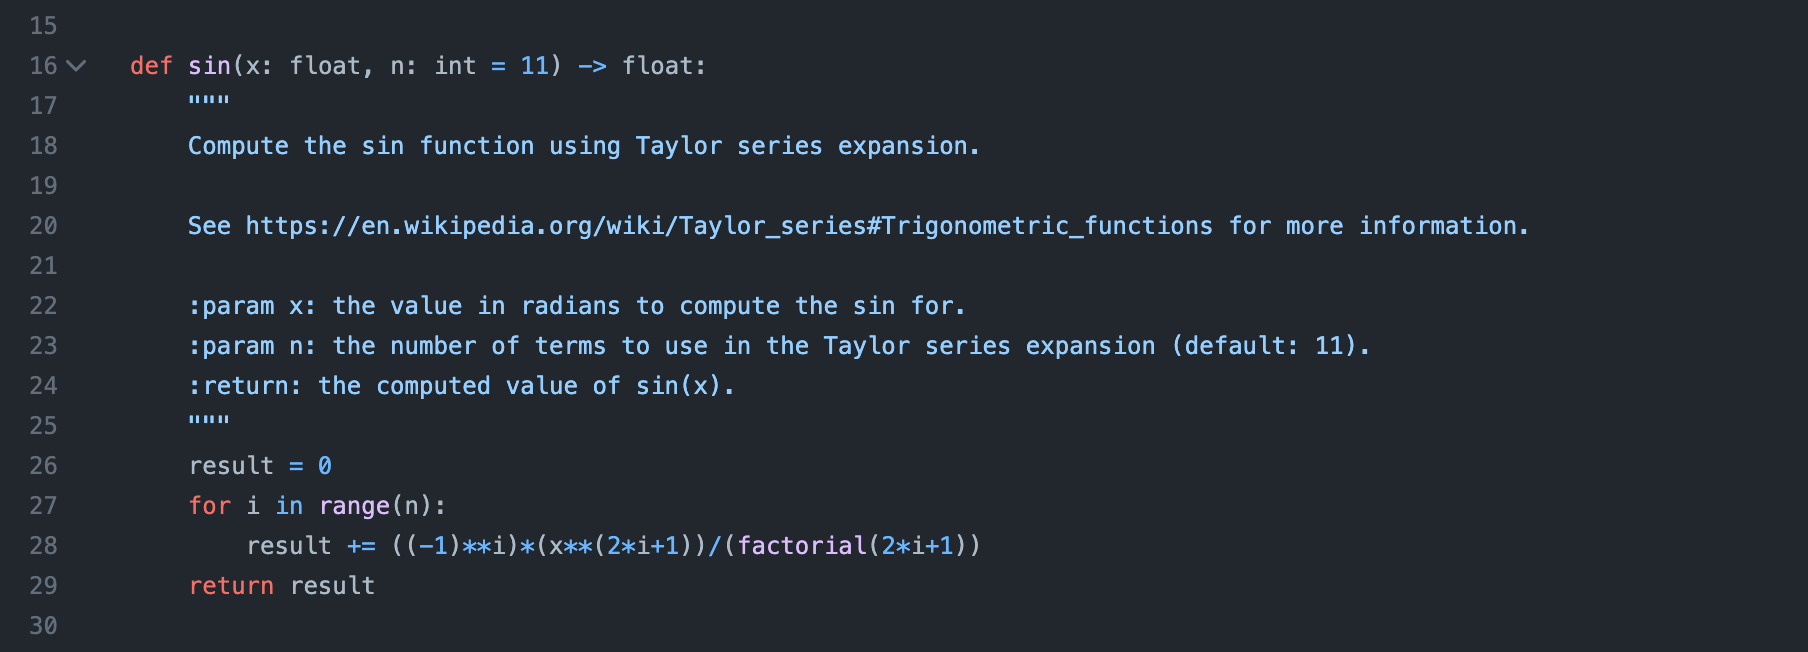
\includegraphics[width=13cm]{images/sin.png}
    \caption{Computed the value of \textbf{sine} using Taylor series}
    \label{fig:sin}
\end{figure}
\begin{figure}[h]
    \centering
    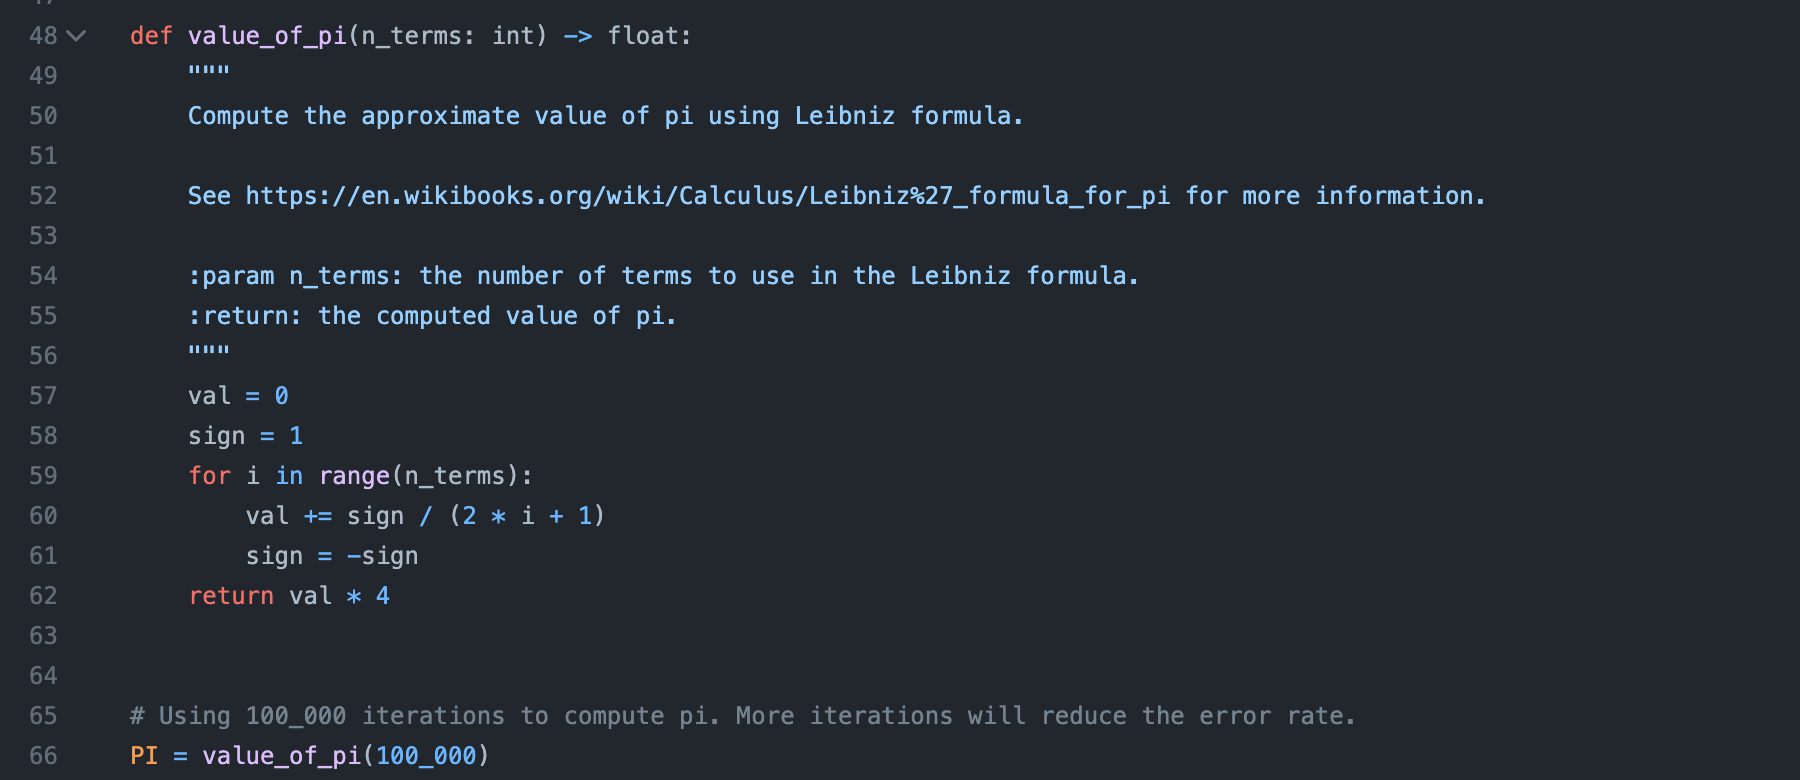
\includegraphics[width=13cm]{images/pi.png}
    \caption{Computed the value of \textbf{pi} using Taylor series}
    \label{fig:pi}
\end{figure}

\begin{figure}[h]
    \centering
    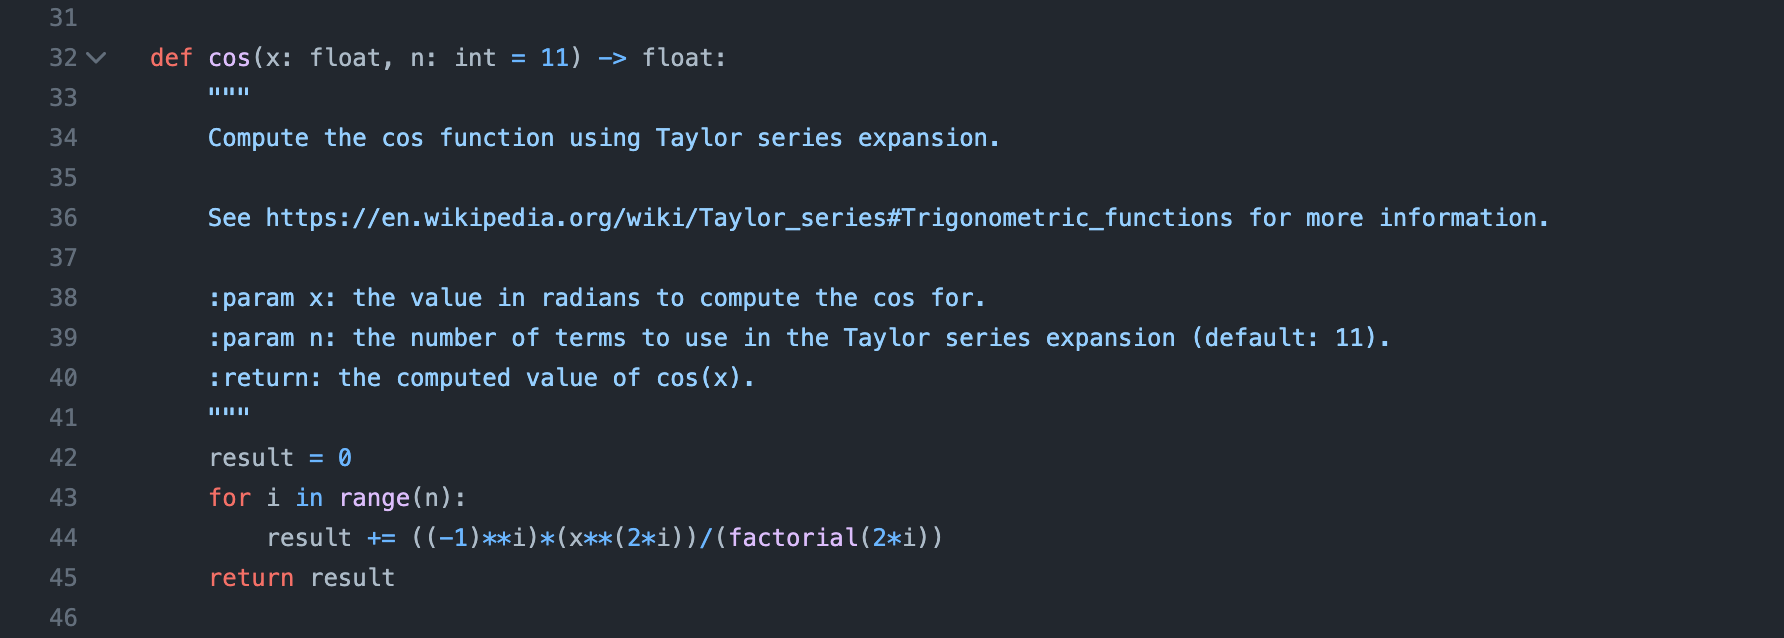
\includegraphics[width=13cm]{images/cos.png}
    \caption{Computed the value of \textbf{cos} using Taylor series}
    \label{fig:cos}
\end{figure}
\newpage
\noindent\large Sample output for different values of R

\begin{figure}[h]
    \centering
    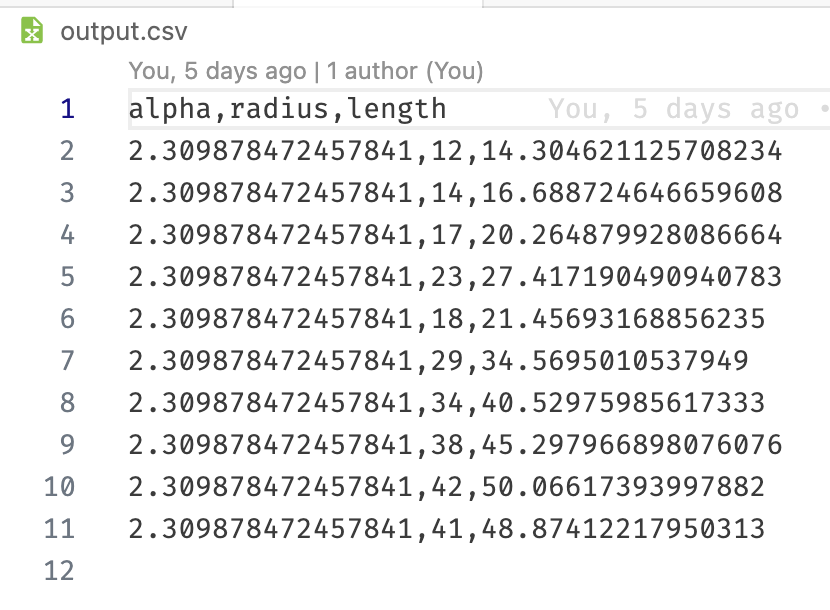
\includegraphics[width=12cm]{images/_CSV.png}
    \caption{Sample output for different values of \textbf{R}}
    \label{fig:csv}
\end{figure}




\section{Incarnation 2}

We have created 2 python files to execute our code. One works with all the inbuilt libraries and the other one with the custom-made libraries.
\\
\\
The libraries we have used are: $Math, Sys, CSV ,IO , Typing and Xml.dom.minidom$

       
\begin{itemize}
    \item \textbf{Math Library}: In order to verify our computed mathematical values with the original one we are using the math library.
    \item \textbf{Sys}: It is used for taking user inputs from keyboard.
    \item \textbf{CSV}: This function is used to extract the length of segment values for various R values and represent it in a CSV file.
    \item \textbf{IO}:  string representing the CSV data.
    \item \textbf{Typing}: From this module we import Tuple ,list so that for every R values we update the list.
    \item \textbf{Xml.dom.minidom}: This module is used for generating XML file for various values of R.
\end{itemize}

\noindent Steps taken towards making S to be readable, modifiable, testable, and understandable after using native libraries:
 \\
 \\
\noindent \textbf{Readability:} We have used clear and descriptive variable names, so that anyone reading the code can quickly understand their purpose.

\noindent Examples: $compute\_alpha$ – is a method to compute the value of alpha. $newton\_method$ - Returns The calculated root value of `func` using Newton's method.\\

\noindent \textbf{Modifiability:} We have broke down our code into smaller parts i.e. dividing the entire code into smaller methods and re using it which allows us to understand and modify the code easily.\\

\noindent\textbf{Understandable}: We have added comments for every piece of code we wrote so that if anyone wants make changes to the code they can understand the functionality from comments.
Example :
The usage of comments in one of our method illustrated below.
We have tested various test cases by providing different r values and examined the results obtained.\\

\noindent\large\textbf{Steps can be taken to ensure that the relevant P is designed to be comprehensive, robust, and applicable:} \\
\newline\textbf{ Generalization:} A method to facilitate adaptation of code based on specific requirements, so less per module A modular system with arguments is to be used. Thus makes it easy to update or design the code according to the user specifications.\\
\textbf{Robustness}: To enhance our  code robustness, we handled every possible exceptions and errors using python exception handling mechanism. This ensures that the code is sufficiently robust and generates informative error messages to users when unsupported arguments are passed.\\
\textbf{Usability} : To increase the usability of the code, we have made it more reusable due to its modular design, which makes it easy to reuse individual modules. Smaller modules make it easier to integrate code with other programs, thus improving its implementation.\\

 \begin{figure}[h]
    \centering
    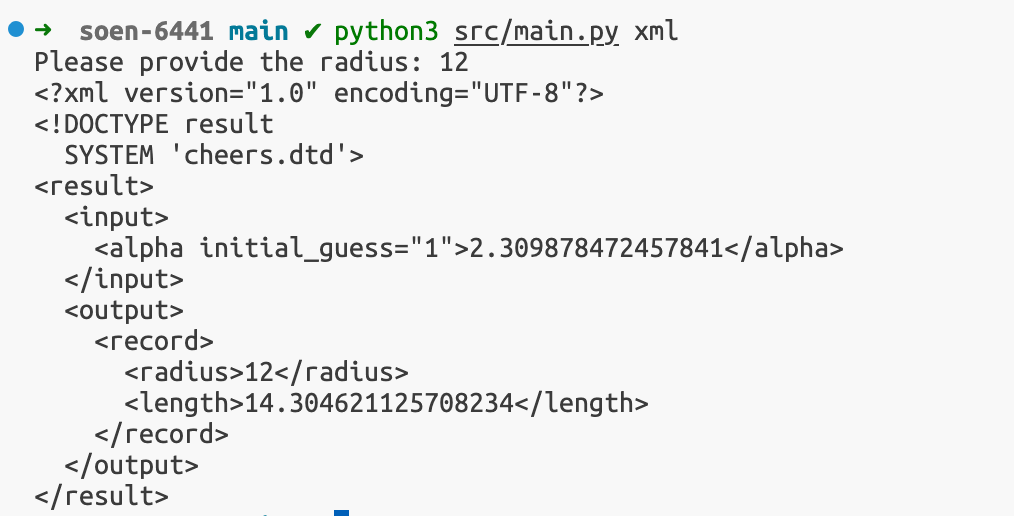
\includegraphics[width=7cm]{images/xml.png}
    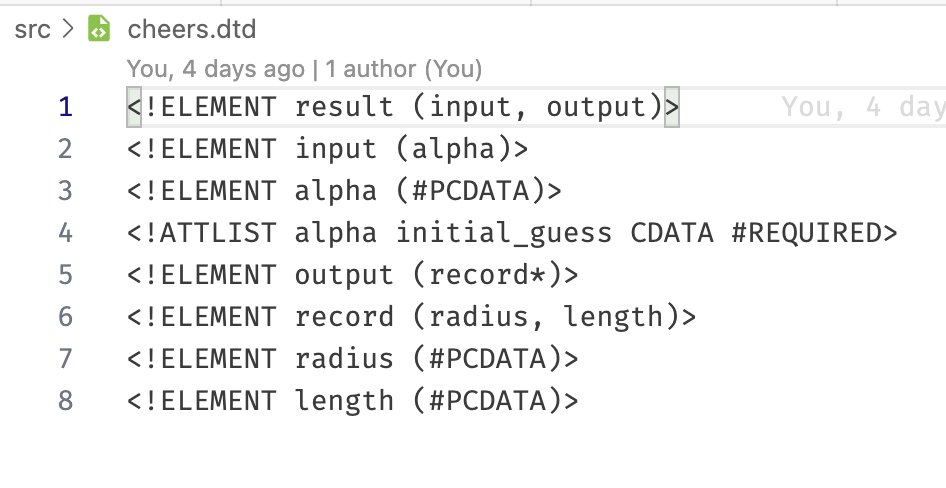
\includegraphics[width=7cm]{images/dtd.png}
    \caption{Sample XML output}
    \label{fig:xml}
\end{figure}
 

\noindent\textbf{Steps taken to Make our S IDE independent :}\\


\noindent 
\begin{itemize}
    \item We have used requirements.txt file , where we listed all the dependencies we have used for our project.
    \item We have avoided the usage of IDE-specific libraries , so that the libraries we use are pre installed along with python installation, which makes our code IDE independent.
    \item To manage our code and dependencies, we have used Git version control.
    \item This enables us to move our code between different environments easily.
    \item Additionally, we have used virtual environments to isolate our code and its dependencies from the system Python installation. This helps to prevent conflicts between different versions of libraries and ensures that our code runs consistently across different environments. 
 
    \begin{figure}[h]
    \centering
    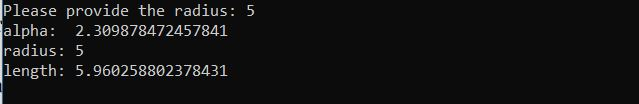
\includegraphics[width=10cm]{images/CMD.png}
    \caption{Output in Command line}
    \label{fig:CMD}
    \end{figure}
    
    \begin{figure}[h]
    \centering
    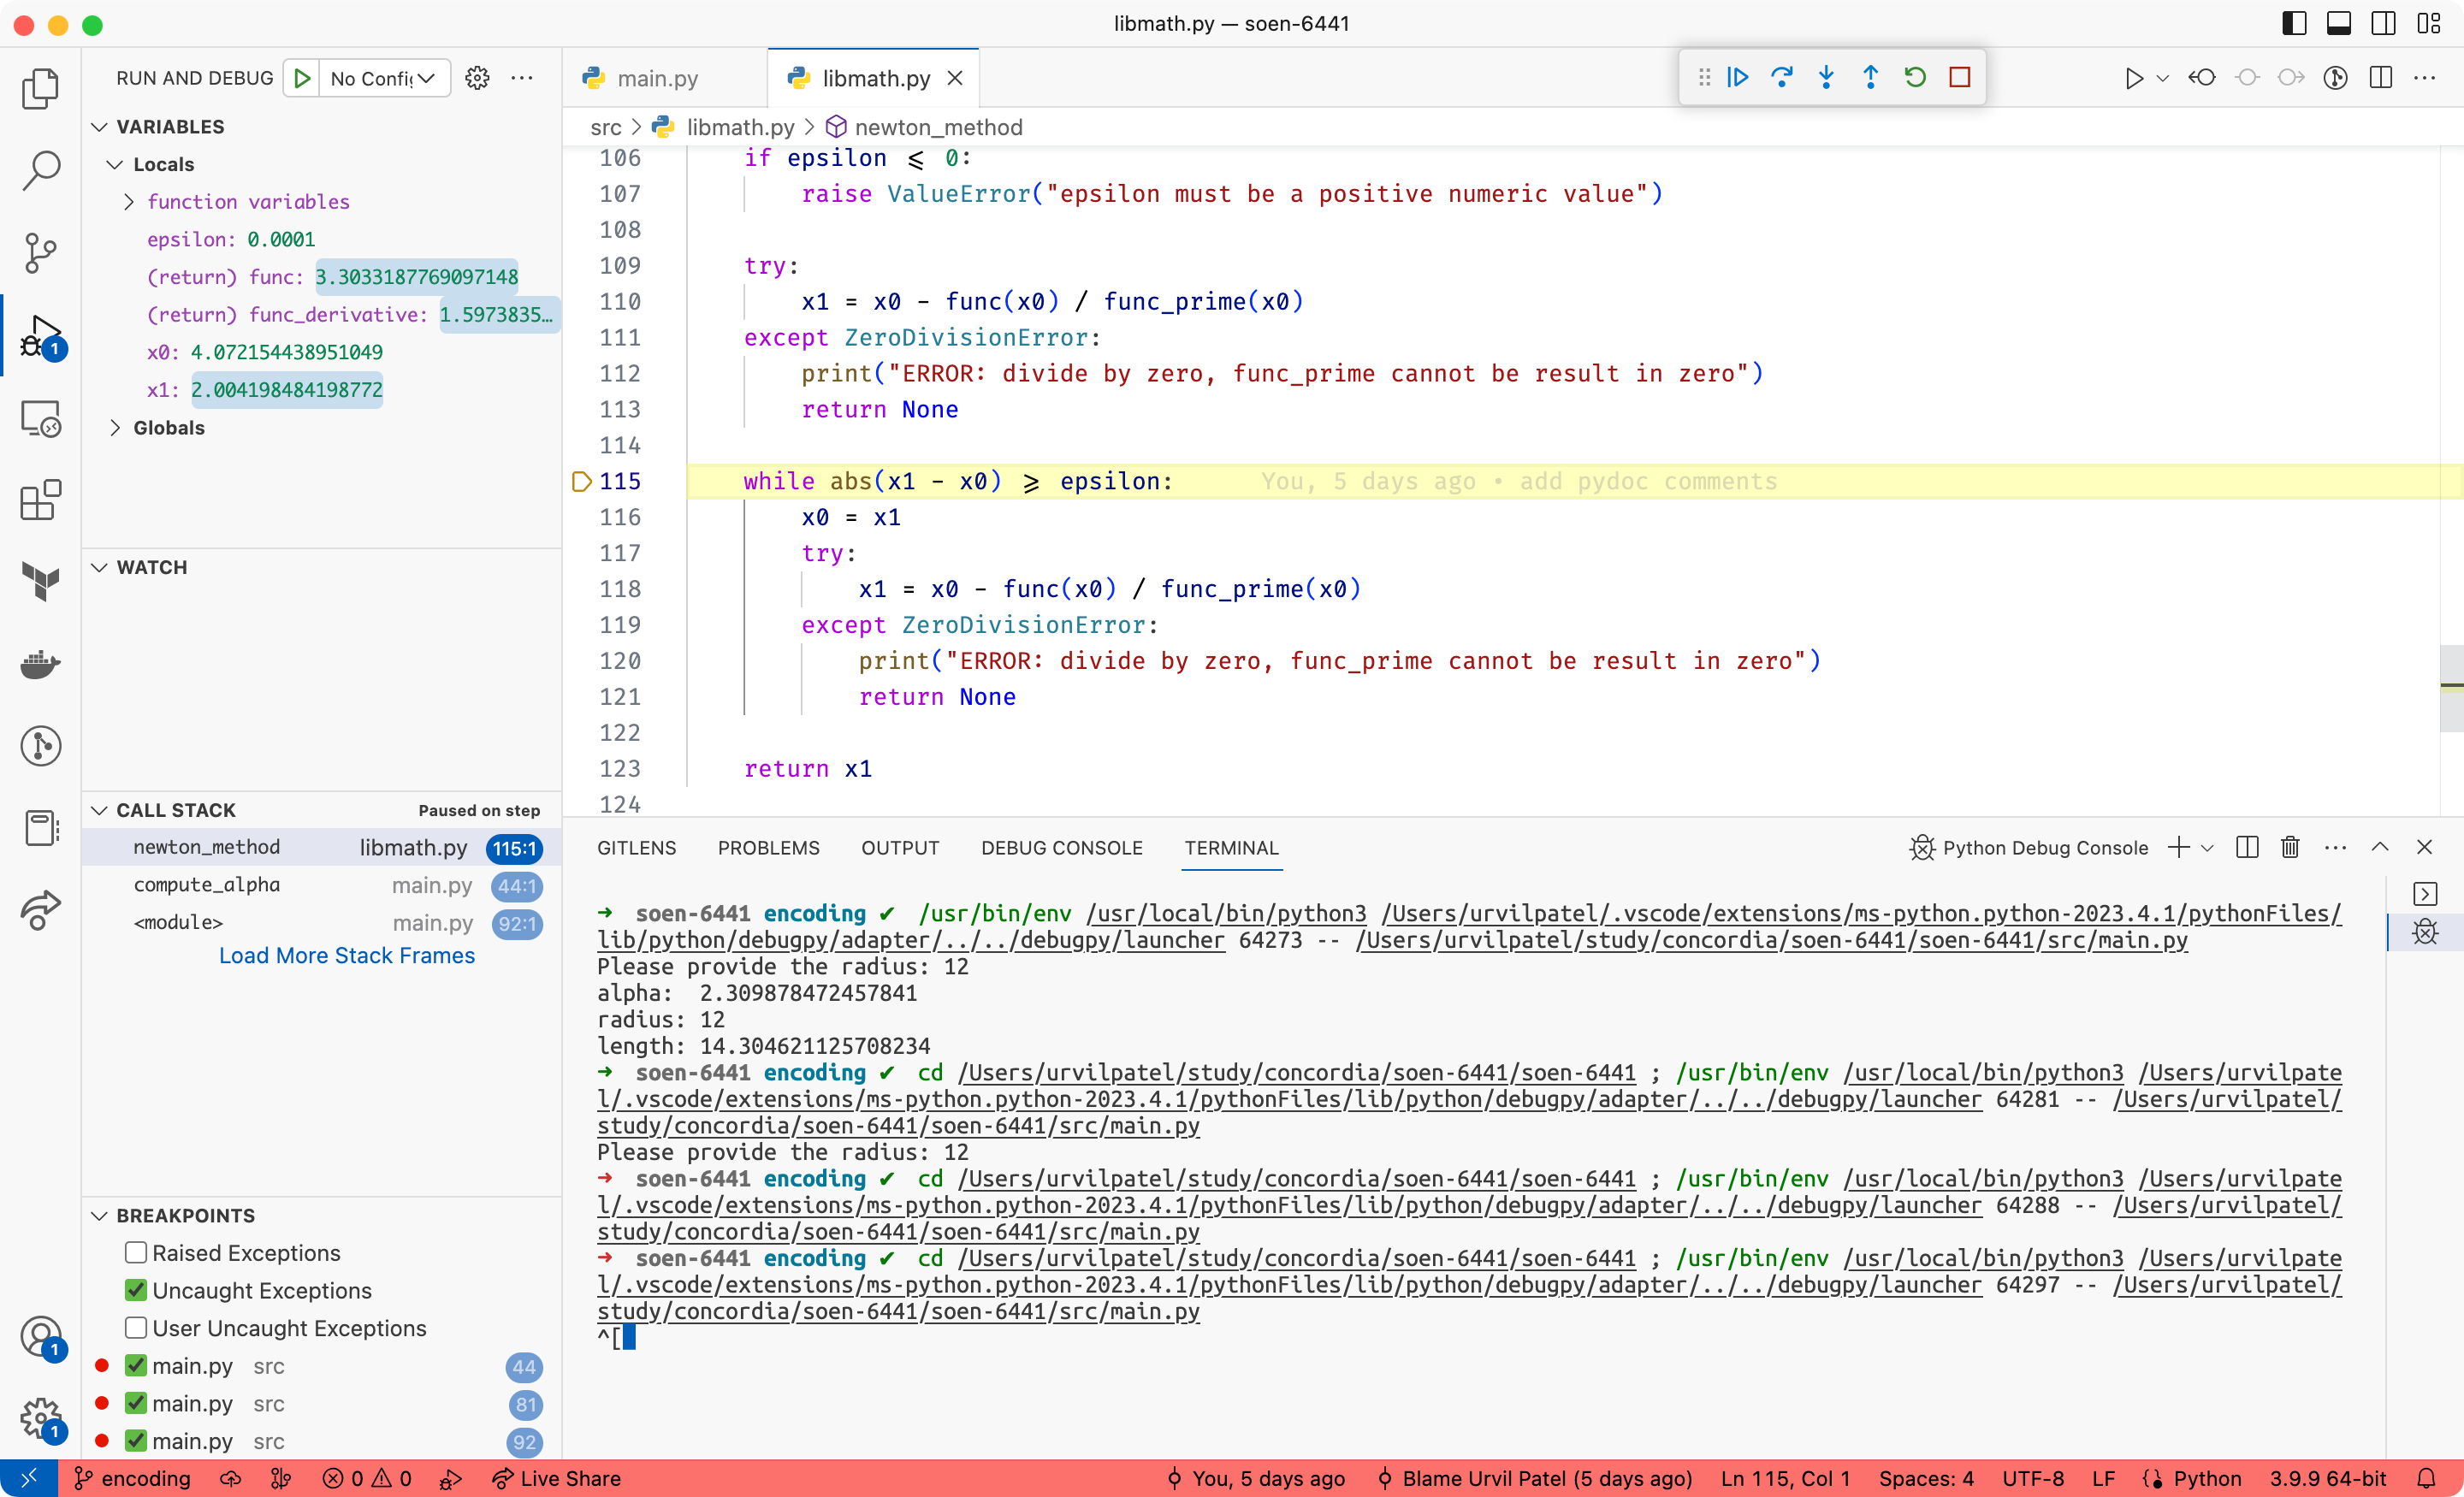
\includegraphics[width=12cm]{images/debugger.png}
    \caption{Usage of Debugger}
    \label{fig:debugger}
    \end{figure}
    \item We have used Pylint for enforcing PEP 8 coding style and to check coding consistency and to improve coding quality.

    \begin{figure}[h]
    \centering
    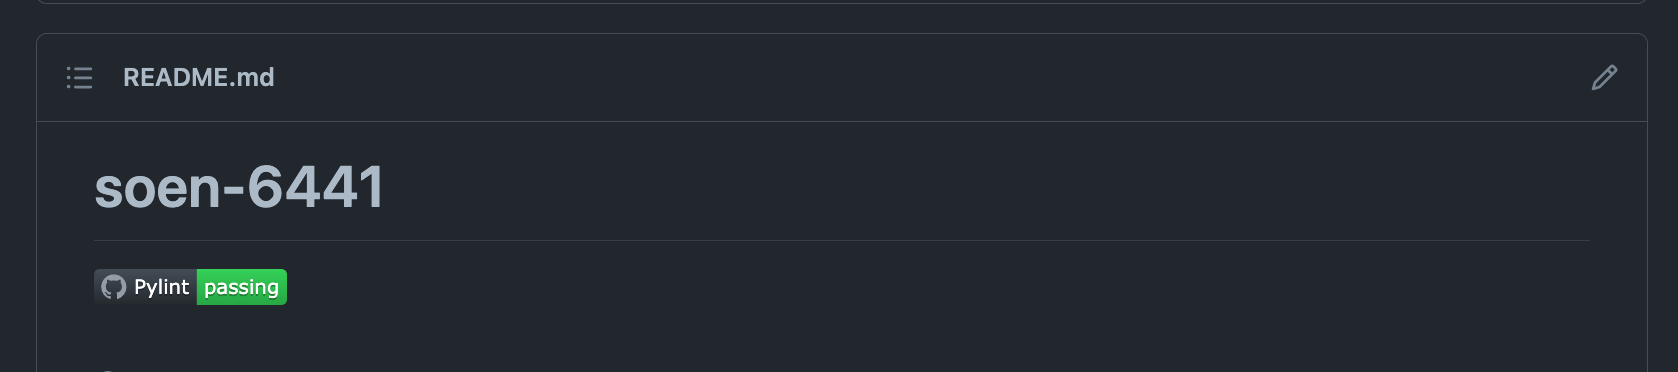
\includegraphics[width=12cm]{images/pylint.png}\\
    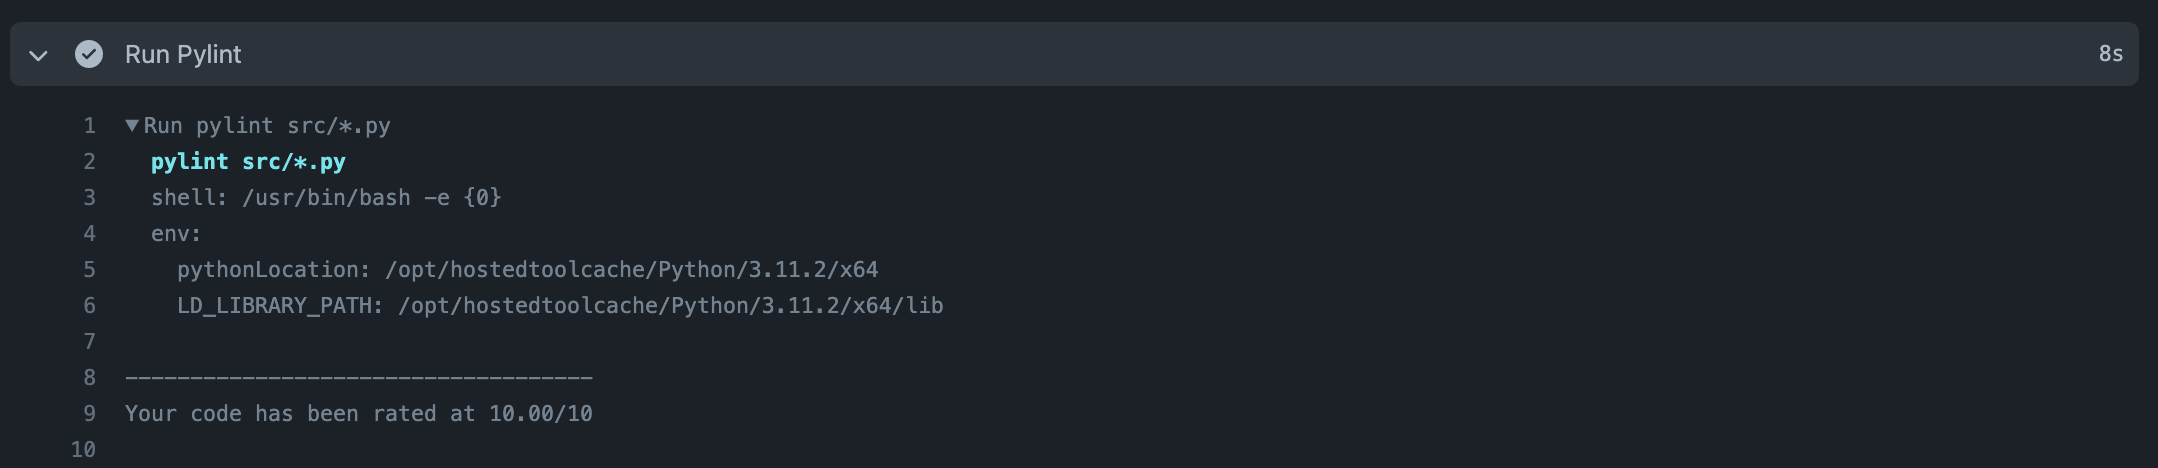
\includegraphics[width=12cm]{images/PEP8.png}
    \caption{Uses of Pylint and PEP8}
    \label{fig:pylint}
    \end{figure}
     
    
    \item In our S we have used a method named compute \_PI(no\_of\_iterations)-  which computes the value of PI without using inbuilt libraries.
    \item Our S has been developed with proper exception and error handling mechanisms using various Error types available in python.
We are using Python debugger module PDB and Pydoc for documentation of the code.\\
\end{itemize}

 \begin{figure}[h]
    \centering
    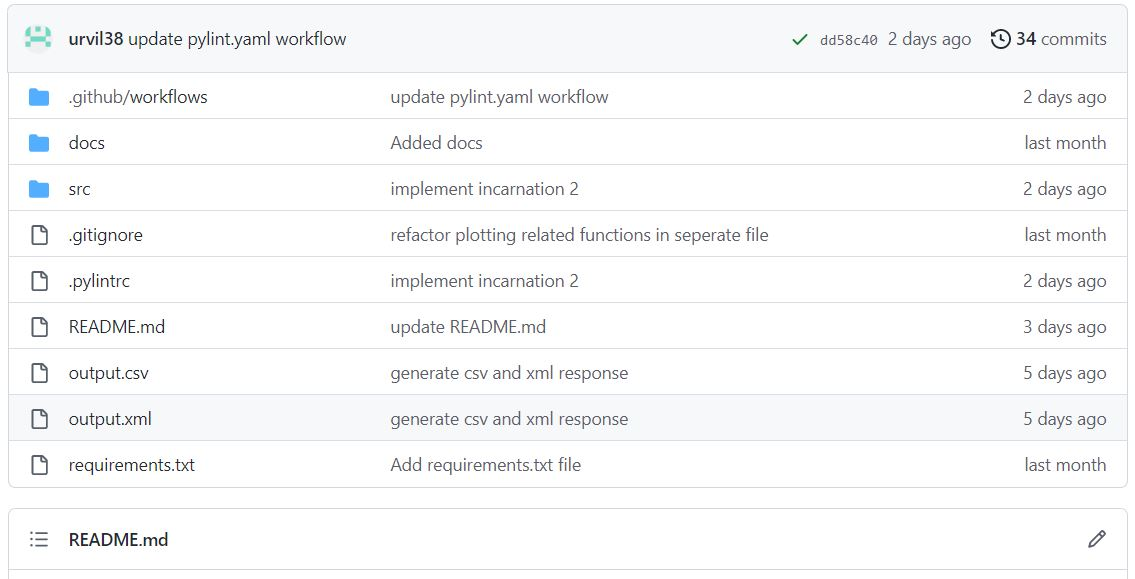
\includegraphics[width=12cm]{images/Github.png}
    \caption{GitHub repository}
    \label{fig:Github}
    \end{figure}


\noindent All our Source code is listed in the link:
\url{https://github.com/urvil38/soen-6441}\\

\noindent Description for Processing Source code: \url{https://github.com/urvil38/soen-6441/blob/main/README.md}


